\section{Solução desenvolvida}\label{sec:solucao-desenvolvida}
Motivado pela demanda de serviços de identificação de pessoas e pelo fato de que as soluções para tal problema ainda permanecem em aberto, este trabalho propõe a utilização de um método ainda recente na área sensorial: a utilização de mapas de profundidade. O mecanismo de identificação consiste em extrair esse mapa através do projetor infravermelho e do sensor monocromático, e analisar os dados obtidos, utilizando de filtros e algoritmos de segmentação. Por fim, é exibida graficamente uma visualização do mapa de profundidade gerado e, em caso de positivo, o(s) indivíduo(s) encontrado(s) na cena. É exibido também os dados que podem ser exportados para plataformas externas: a localização aproximada dos sujeitos no plano 3D (posições $X$, $Y$ e $Z$) e a distância em relação ao \textit{Kinect}. Nesta seção é discutida a solução desenvolvida.



\subsection{Arquitetura da solução}\label{sec:arqSol}
O \textit{Kinect} será responsável por obter a visualização da cena de um ambiente interno. Como discutido na seção \ref{sec:trabalhos-relacionados}, o \textit{Kinect} é um sensor de movimento muito eficiente, extraindo com precisão objetos, pessoas e detalhes de uma cena. A \textit{Microsoft} provê para o \textit{Kinect} um Kit de desenvolvimento de software (\textit{Software Development Kit}, SDK).O sistema é composto por módulos adicionados à camada de aplicação, Sobre a camada do SDK. A Figura \ref{fig:visao-geral} apresenta uma visão geral da solução.
 
\begin{figure*}[ht]
\centering
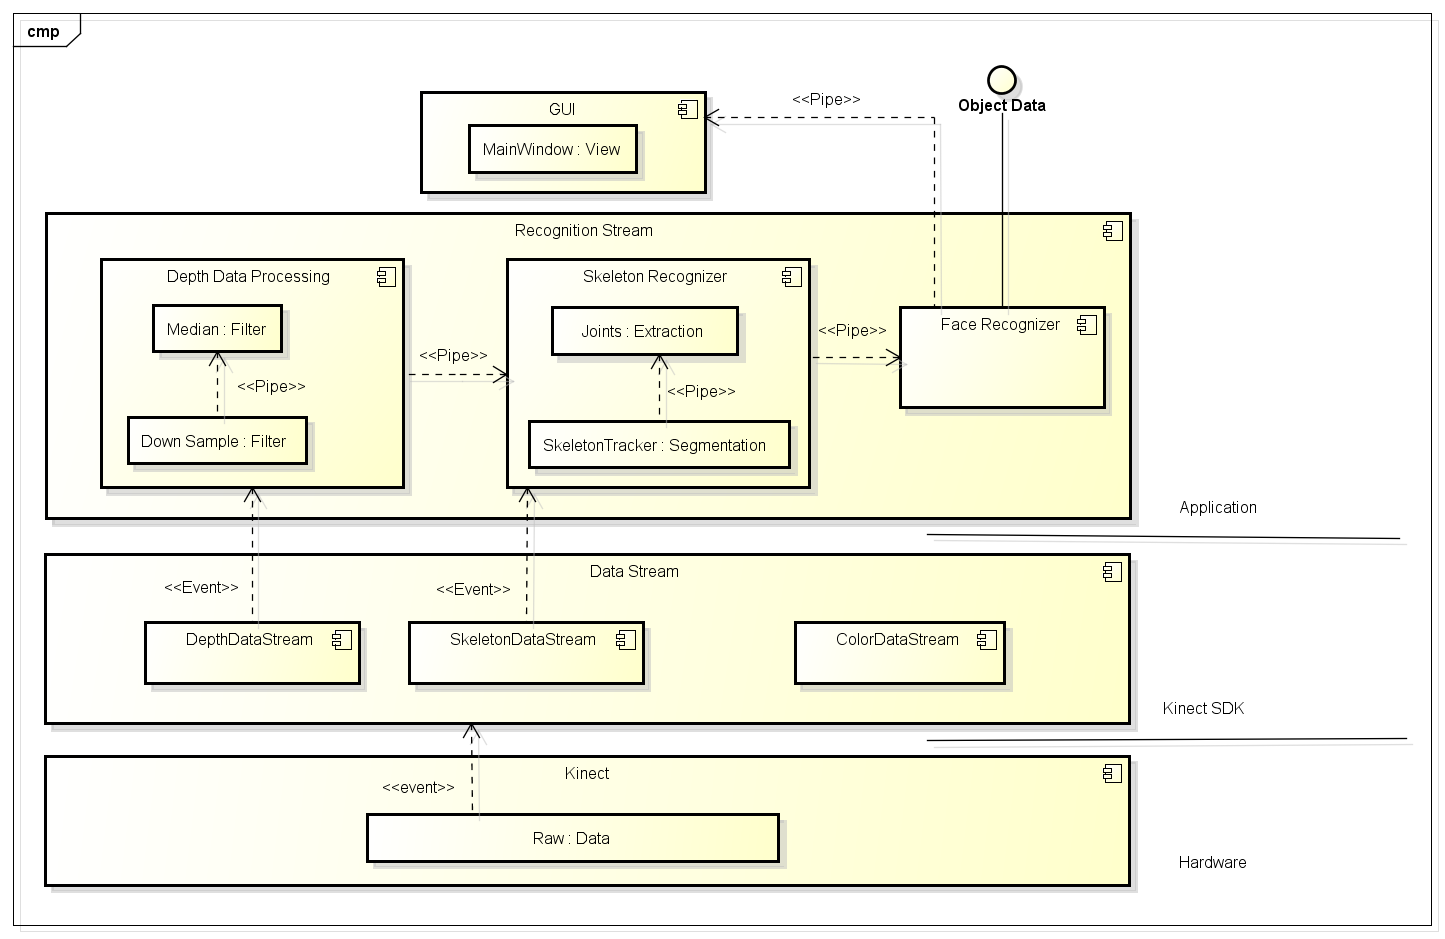
\includegraphics[width=1.0\textwidth]{images/Arquitetura_da_solucao.png}
\caption{Arquitetura da solução proposta}
\label{fig:visao-geral}
\end{figure*}


\subsubsection{Estilos arquiteturais}\label{sec:estilosArq}
A solução apresenta um estilo arquitetural híbrido, com características de três estilos arquiteturais básicos:

\begin{itemize}
\item Baseado em invocação implícita: \textit{Event Based}; 
\item Baseado em fluxo de dados: \textit{Pipe and Filter}; 
\item Em camadas: \textit{Virtual Machine}.
\end{itemize}

O estilo baseado em eventos (\textit{Event Based}) é um estilo arquitetônico baseado na invocação implícita que fornece uma interação indireta entre componentes acoplados de forma livre, facilitando a adaptação e melhorando a escalabilidade do sistema. Os componentes do tipo de evento (\textit{Depth}, \textit{color} e \textit{Infrared}.) comunicam-se apenas através de eventos transmitidos por um conector de evento.
Este conector então retransmite os eventos para todos os componentes do tipo \textit{Observer} mostrando interesse no evento em questão (Nesse caso, o \textit{Recognition Stream}), melhorando assim a eficiência da distribuição de eventos.


\textit{Pipes} e Filtros (\textit{Pipe and Filter}) é um estilo arquitetural composto por uma cadeia de elementos de processamento, dispostos de forma tal que a saída de cada elemento é a entrada do próximo. O fluxo de dados se dá através de \textit{pipes} (canos) e os dados sofrem transformações quando processados nos filtros. Em outras palavras, os \textit{pipes} é que possibilitam o fluxo dos dados, e os filtros fazem o processamento dos mesmos, colocando-os nos \textit{pipes} antes que todos os dados de entrada sejam consumidos. Portanto, a nível de arquitetura, o processamento é mapeado em filtros e os \textit{pipes} agem como condutores de dados. O componente \textit{Recognition Stream} é composto por subcomponentes do tipo \textit{Filter} e a comunicação entre os mesmos se dá através dos conectores do tipo \textit{Pipe}. 

As arquiteturas de máquinas virtuais (\textit{Virtual Machines}) têm como objetivo alcançar a qualidade da portabilidade. Este estilo de arquitetural simula algumas funcionalidades que não são originais para o \textit{hardware} e/ou \textit{software} em que é implementado. O estilo é aplicado entre o \textit{Kinect (hardware)} e a aplicação desenvolvida, usando conectores do tipo \textit{Event} e \textit{Pipe} entre as camadas. Esse estilo arquitetônico reduz a complexidade, melhora a modularidade, reutilização e manutenção.
Conforme visto na figura \ref{fig:visao-geral}, o sistema possui as camadas:

\begin{itemize}
\item \textit{Kinect (hardware)};
\item \textit{Kinect} SDK; 
\item Aplicação; 
\end{itemize}


\subsubsection{Arquitetura do \textit{Kinect for Windows} SDK}\label{sec:kinectSDK}
O SDK fornece uma biblioteca e ferramentas de software sofisticadas para ajudar os desenvolvedores a usar a forma rica de entrada natural baseada no uso do \textit{Kinect}, que detecta e reage a eventos do mundo real. O \textit{Kinect} e a biblioteca de software interagem com aplicações, como mostrado na Figura \ref{fig:sdk_interact}. Os componentes do SDK são exibidos na figura \ref{fig:sdk_architecture_color} e incluem:

\begin{figure}[h]
\centering
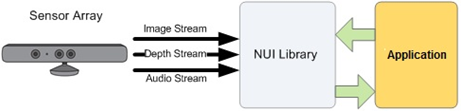
\includegraphics[width=0.5\textwidth]{images/sdk_interaction.png}
\caption{Interação de Hardware e Software com a Aplicação}
\label{fig:sdk_interact}
\end{figure}


\begin{figure*}[ht]
\centering
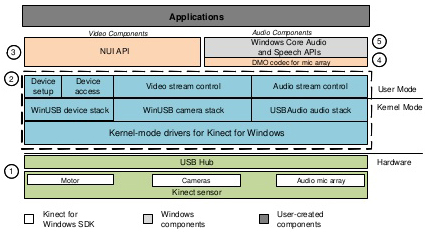
\includegraphics[width=0.8\textwidth]{images/sdk_architecture_color.png}
\caption{Arquitetura do SDK}
\label{fig:sdk_architecture_color}
\end{figure*}

\begin{enumerate}
    \item \textit{Hardware Kinect} - Os componentes de \textit{hardware}, incluindo o sensor \textit{Kinect} e o \textit{hub} USB através dos quais o sensor \textit{Kinect} está conectado ao computador;
    \item \textit{Drivers Kinect} - Os \textit{drivers} do Windows para o \textit{Kinect}, que são instalados como parte do processo de configuração do SDK. Os \textit{drivers} do \textit{Kinect} suportam:
        \begin{itemize}
            \item A matriz de microfones como um dispositivo de áudio em modo \textit{kernel} que pode ser acessado  através das API de áudio padrão no Windows; 
            \item Controles de transmissão de áudio e vídeo para transmissão de áudio e vídeo (cor, profundidade e esqueleto);
            \item Funções de enumeração de dispositivos que permitem que um aplicativo use mais de um \textit{Kinect}.	
        \end{itemize} 
    \item Componentes de Áudio e Vídeo:
        \begin{itemize}
            \item Interface de usuário natural do Kinect para rastreamento de esqueleto, áudio e imagem em cores e profundidade. 
        \end{itemize}
    \item Objeto de mídia DirectX (DMO) para formatação de feixes de microfone e localização de fonte de áudio;
    \item API padrão do Windows - APIs de áudio, voz e mídia no Windows, conforme descrito no SDK do Windows e no Microsoft \textit{Speech} SDK.
\end{enumerate}


\subsection{Componentes principais}\label{sec:componentes}

\subsubsection{Color Data Stream}\label{sec:colorDataStream}

\subsubsection{Depth Data Stream}\label{sec:depthDataStream}
capturing data stream

\subsubsection{Skeleton recognizer }\label{sec:skeleton}
processing joints

\subsubsection{Depth Data Processing (Recognition Stream - Filter)}\label{sec:depthDataProcessing}
processing data stream



\subsubsection{Face Recognition (Recognition Stream )}\label{sec:depthDataRecognition}
processing data stream